\documentclass{emulateapj}
%\documentclass{aastex}
\submitted{{\it Submitted for publication in ApJ}}
\usepackage {graphicx}

\usepackage{amsmath}
\usepackage{amssymb}
\usepackage{graphics}
\usepackage{epsfig}
\usepackage{float}
\bibliographystyle{apj}
\def\be{\begin{equation}}
\def\ee{\end{equation}}
\def\ba{\begin{eqnarray}}
\def\ea{\end{eqnarray}}


\newcommand{\documentname}{paper~}
\newcommand{\match}{{\tt match}~}
\newcommand{\kms}{\,km~s$^{-1}$}
\def\squig{\sim\!\!}
\newcommand{\LCDM}{$\Lambda$CDM~}
\newcommand{\beq}{\begin{eqnarray}}  
\newcommand{\eeq}{\end{eqnarray}}   
\newcommand{\zz}{$z\sim 3$} 
\newcommand{\avg}[1]{\langle{#1}\rangle}  
\newcommand{\ly}{{\ifmmode{{\rm Ly}\alpha}\else{Ly$\alpha$~}\fi}}
\newcommand{\hMpc}{{\ifmmode{h^{-1}{\rm Mpc}}\else{$h^{-1}$Mpc }\fi}}  
\newcommand{\hGpc}{{\ifmmode{h^{-1}{\rm Gpc}}\else{$h^{-1}$Gpc }\fi}}  
\newcommand{\hmpc}{{\ifmmode{h^{-1}{\rm Mpc}}\else{$h^{-1}$Mpc }\fi}}  
\newcommand{\hkpc}{{\ifmmode{h^{-1}{\rm kpc}}\else{$h^{-1}$kpc }\fi}}  
\newcommand{\hMsun}{{\ifmmode{h^{-1}{\rm
        {M_{\odot}}}}\else{$h^{-1}{\rm{M_{\odot}}}$}\fi}}   
\newcommand{\hmsun}{{\ifmmode{h^{-1}{\rm
        {M_{\odot}}}}\else{$h^{-1}{\rm{M_{\odot}}}$}\fi}}   
\newcommand{\Msun}{{\ifmmode{{\rm {M_{\odot}}}}\else{${\rm{M_{\odot}}}$}\fi}}  
\newcommand{\msun}{{\ifmmode{{\rm {M_{\odot}}}}\else{${\rm{M_{\odot}}}$}\fi}}  
\newcommand{\clara}{{\texttt{CLARA}}~}
\newcommand{\rand}{{\ifmmode{{\mathcal{R}}}\else{${\mathcal{R}}$ }\fi}}  
\newcommand{\Lsun}{\mbox{\,$L_{\odot}$}}
\newcommand{\like}{\mathscr{L}}
\newcommand{\bftheta}{\mathbf{\Theta}}
\newcommand{\degree}{\ensuremath{^\circ}}
\def\spose#1{\hbox to 0pt{#1\hss}}
\def\simlt{\mathrel{\spose{\lower 3pt\hbox{$\mathchar"218$}}
     \raise 2.0pt\hbox{$\mathchar"13C$}}}
\def\simgt{\mathrel{\spose{\lower 3pt\hbox{$\mathchar"218$}}
     \raise 2.0pt\hbox{$\mathchar"13E$}}}
\font\smcap=cmcsc10

\begin{document}


\title{The impact of cosmic variance on constraining the mass and
  occupation fraction of dark matter halos hosting Lyman-$\alpha$
  emitters at $z \sim 3$}      
\author{
  Jaime E. Forero-Romero$^{1}$ and
  Julian E. Mej\'ia-Restrepo$^{2,3}$ 
}

\affil{
$^{1}$ Departamento de F\'{i}sica, Universidad de los Andes, Cra. 1
No. 18A-10, Edificio Ip, Bogot\'a, Colombia \\
$^{2}$ Departamento de Astronom\'{i}a, Universidad de Chile, Camino el
Observatorio 1515, Santiago, Chile\\
$^{3}$ FACom-Instituto de F\'isica-FCEN, Universidad de Antioquia, Calle 70 No. 52-21, Medell\'in, Colombia
} 



\begin{abstract}
%
  We study the impact of cosmic variance in constraining the mass and
  occupation fraction of dark matter halos hosting \ly Emitting
  Galaxies at high redshift. We use an N-body simulation to construct
  mock fields with the same typical size of observed fields at
  $z=3.1$ to match the observed number density distribution across
  fields and the angular correlation function. In our model a dark
  matter halo with mass in the range $M_{\rm min}<M_{\rm h}<M_{\rm
    max}$ can only host one detectable LAE with a probability $0.1
  \leq f_{\rm occ}\leq 1.0$.  Our analysis shows that the clustering
  and number density information are insufficient to impose a tight
  constraint on the occupation fraction. On the other hand, the
  minimum mass and maximum mass can be constrained to the range
$10^{10.2}\hMsun\leq M_{\rm min}\leq 10^{11.5}\hMsun$ and $M_{\rm  max}<10^{12}$\hMsun.
Additionally, we find that the
  consistent models have a narrow mass range, $\Delta M \equiv \log_{10}M_{\rm max} -
  \log_{10} M_{\rm min}$, smaller than $1.0$ dex, with a majority in
  the range $\Delta M<0.5$ dex. These results fall into constraints
  already presented in the literature. However, the wide range of
  values for the occupation fraction and the narrow mass range $\Delta
  M$ are novel results allowed by taking into account the influence of
  cosmic variance on the statistics derived from observations.  
\end{abstract}


\keywords{cosmology: theory, dark matter --- methods: numerical --- galaxies: formation --- galaxies: high-redshift}



\section{Introduction}

Lyman-$\alpha$ emitting galaxies (LAEs) are helpful in a diverse range
of subjects in extragalactic astronomy. LAEs can be
used as probes of reionization \citep{Dijkstra11}, tracers of large
scale structure \citep{Koehler2007},  signposts for low metallicity
stellar populations, markers of the galaxy formation process at high
redshift \citep{Dayal2009,ForeroRomero2012} and tracers of active star
formation \citep{Guaita2013}. 

Capitalizing LAEs observations requires an understanding of
their place in structure formation model in an explicit cosmological
context. Under the current paradigm the dominant matter content of the
Universe is to be found in dark matter (DM) and each galaxy is thought
to be hosted by a larger dark matter structure known as a
halo. \citep{Peebles1980,SpringelNature05}.  

Galaxy formation models find that halo mass predicts with high
accuracy galactic properties such as stellar mass and star formation
rate \citep{Behroozi2013a}. This suggests that the
physical processes that regulate the star formation cycle are 
dependent on halo mass.  For that reason, finding the typical dark
matter halo mass hosting LAEs represents an advance to understand the
nature of this galaxy population in the context of Lambda Cold Dark
Matter ($\Lambda$CDM) paradigm.  

There are theoretical attempts to solve this problem using an  ab-initio
approach. They start from the DM halo population to infer the
intrinsic star formation rates and \ly  luminosities. From these
values they estimate the amount of \ly photons that
escape each galaxy and compute the observed luminosity for each
galaxy. These models can predict different observables including: the
luminosity function, correlation function and the equivalent width
distributions. Such modelling has been implemented in semi-analytic
models \citep{Garel2012,Orsi2012} and  full N-body
hydrodynamical simulations \citep{Laursen2007, Dayal2009,
  ForeroRomero2011, Yajima2012}. 

However, these calculations involve many uncertain steps such as 
the estimation of the escape fraction of \ly photons. Given the resonant
nature of the \ly line, the escape fraction is sensitive to  the dust
contents, density, temperature, topology and kinematics of the neutral
Hydrogen in the interstellar medium (ISM). Solving the radiative
transfer of \ly photons in the ISM requires Monte Carlo
simulations. The process of finding a consensus on the expected value
for the \ly escape fraction in high redshift galaxies is still matter
of ongoing research
\citep{Neufeld1991,Verhamme2006,ForeroRomero2011,Dijkstra2012,Laursen2013,Orsi2012}.

A different approach to infer the typical mass of halos hosting
LAEs is based on the spatial clustering information. This approach uses the fact
that in CDM cosmologies the spatial clustering of galaxies on large
scales is entirely dictated by the halo distribution
\citep{Colberg00}, which in turn has a strong dependence on halo
mass. Using measurements of the angular correlation function of LAEs,
observers have put constraints on the typical mass and occupation
fraction of the putative halos hosting these galaxies
\citep{Hayashino2004,Gawiser07,Nilsson2007,Ouchi2010}. In these
studies the observations are done on fields of $\sim 1$ deg$^{2}$ and
the conclusions derived on the halo host mass do not delve too deeply
into the possible impact of cosmic variance in their estimates.  

Recently \cite{Yamada2012} observed a wide area of $2.4$ deg$^{2}$
under homogeneous instrumental and data reduction conditions. This data
set is constructed from 12 different sub-fields that allows us to use
clustering statistics and the cosmic variance among fields to
constrain the mass and occupation fraction of halos hosting LAEs. 

In this paper we investigate the impact of cosmic variance in
constraining the mass and occupation fraction of halos hosting LAEs.
We do this by constructing mock catalogs from cosmological simulations.
Our method populates each halo in the simulation with a LAE without
predicting a \ly  luminosity. This bypasses all the physical
uncertainties associated to star formation and radiative transfer.
We build mock surveys following the geometry of the observed fields by
\cite{Yamada2012} to compare them  against observations in terms of
the number density distribution and the angular correlation
function. This allows us to find the range of parameters in our model
that are consistent with observations while taking explicitly into
account cosmic variance. 
  

This \documentname is structured as follows. In the next section we present
the simulation and the model used to produce the mock catalogs. We
also list the criteria used to compare the mocks against
observations. In \S \ref{sec:results} we present the main results for
the halo mass and occupation fraction. We continue in \S
\ref{sec:discussion} with a discussion of other constraints already
presented in the literature and theoretical considerations. Finally,
we present our conclusions in \S \ref{sec:conclusions}.

Throughout this \documentname we assume a $\Lambda$CDM cosmology with the
following values for the cosmological parameters, $\Omega_{m}=0.27$,
$\Omega_{\Lambda}=0.73$ and $h=0.70$, corresponding to the matter
density, vacuum density and the Hubble constant in units of 100 km
s$^{-1}$ Mpc$^{-1}$. 

\section{Methodology}

Our method is based on the comparison of observations and mock
catalogs. This approach explicitly takes into account cosmic
variance. Our benchmarks are the distribution of the surface number
density across fields and the angular correlation function.

In the next subsections we describe in detail the four key
elements in our work-flow. First, we present the 
observations we take as a benchmark. Second, we describe the main
characteristics of the N-body simulation and the halo catalogs we
use. Third, we list the important parameters of the simplified
model that we use to populate the halo catalogs with LAEs. Finally, we
describe the statistical tests we adopt to compare observations and mocks.

\subsection{Observational constraints}


\begin{figure}
\begin{center}
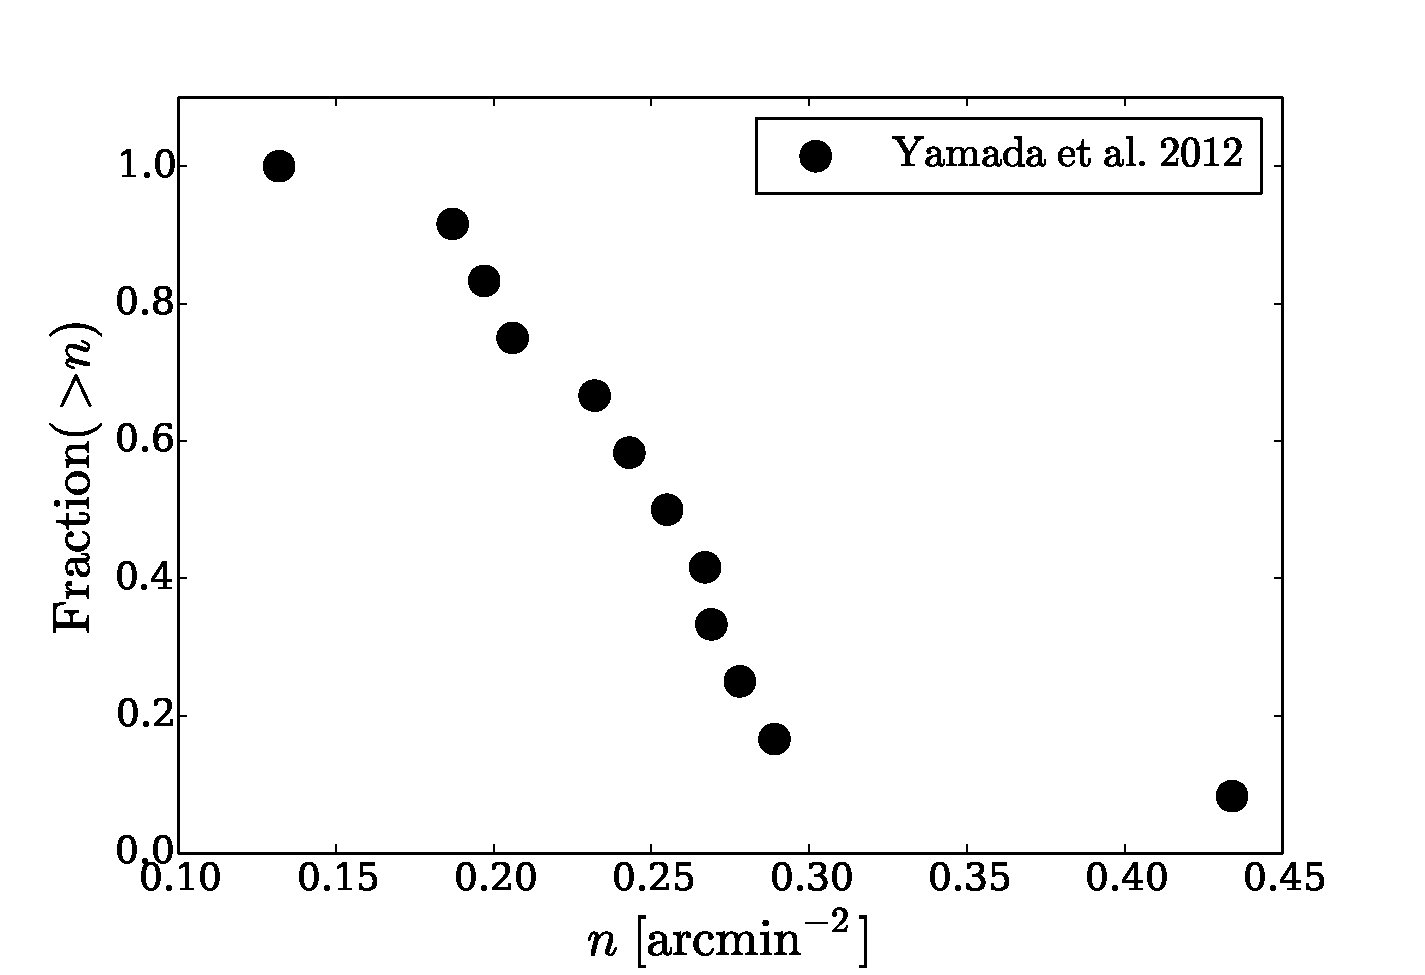
\includegraphics[width=0.95\linewidth,angle=0]{Fig1b.pdf}
\caption{ \label{fig:number_density} Cumulative distribution of LAE number
  densities in all the fields observed by \citet{Yamada2012}. The
  point with the highest surface density corresponds to the densest
  sub-field in the SSA22 field.}
\end{center} 
\end{figure}

The first observational constraint we use in this paper is the LAE number
density information at $z=3.1$ obtained by \cite{Yamada2012} from a survey
conducted with the Subaru 8.2m telescope and the Subaru Prime Focus Camera.
The camera has a field of view covering $34\times 27$ arc-min,
corresponding approximately to a comoving scale of $46\times35$ Mpc
$h^{-1}$ at $z=3.09$.  

The narrow band filter used in the survey is
centered at $4977$ \AA~with  $77$ \AA~width, corresponding to the
redshift range $z=3.062$-$3.125$ and approximately $41$ \hMpc comoving scale for the
detection of the Lyman-$\alpha$ line centered at
$z=3.09$. The authors reported a total of $2161$  LAEs with an
observed equivalent width, in the observer frame, larger than $190$
\AA~over a total survey area of $2.42$ deg$^{2}$ that includes 12
sub-fields,  this corresponds to an average surface number density of
$0.24\pm 0.01$ arcmin$^{-2}$.  The distribution of the surface number
densities is shown in Figure \ref{fig:number_density}.  

The survey covered four independent fields:

\begin{enumerate}
\item The SSA22
field of $1.38$ deg$^2$ with $1394$ detected LAEs. This large field is
composed by 7 sub-fields. 

\item The Subaru/{\it
  XMM-Newton} Deep Survey (SXDS)-North, -Center and -South fields, with a
total of $0.58$ deg$^2$ and $386$ LAEs (3 sub-fields).

\item The Subaru Deep Field (SDF) with $0.22$ deg$^2$ and
$196$ LAEs (1 sub-field).

\item The Great Observatory Optical Deep Survey  (GOODS-N) field with
  $0.24$ deg$^2$ and $185$ LAEs (1 sub-field).   
\end{enumerate}

The surface number density distribution for these fields is shown in
Figure \ref{fig:number_density}.

There is abundant observational work done on LAEs at redshift $z=3.1$
\citep{Kudritzki2000,Matsuda2005,Gawiser2007,Nilsson2007,Ouchi2008}.
However, we use the data from \cite{Yamada2012} because
it has the largest covered area with homogeneous instrumentation
conditions (telescope, narrow band filter), data reduction pipeline
and conditions to construct the LAE catalog. This ensures that the
number density variations among fields are not due to different
observational conditions or criteria to construct the catalogs.

The second benchmark is the angular correlation function
(ACF). Unfortunately, \cite{Yamada2012} do  not report an ACF measurement for
their fields. Instead, we use the results by   \cite{Ouchi2008} who
reported the ACF  over a region of $1$ deg$^2$ over the SXDS
field.  

There are some differences between \cite{Ouchi2008} observations
and those by \cite{Yamada2012}. The details in the color selection,
corresponding limiting luminosities and EW thresholds are different
in these references. In the case of
\cite{Ouchi2008} the number density is $0.099\pm0.005$ arcmin$^{-2}$, which
is 50\% lower that the median value of $0.20$ arcmin$^{-2}$ for the
the general fields in \cite{Yamada2012}. In spite of these
differences \cite{Ouchi2008} provides the most similar conditions
to the observations presented by \cite{Yamada2012}.


We note that the field SSA22-1 has been known to harbor a significant
galaxy overdensity. \cite{Yamada2012} estimates that the densest
sub-field is likely to be a rare density peak with $3-4\sigma$
significance on the scale of $\sim 60$\hMpc.  All the other sub-fields
in SSA22 are average with similar number density as other blank fields. 

From Figure \ref{fig:number_density}  it is evident that there is only
one sub-field  that stands out as an outlier in the distribution,
corresponding to SSA22-1. All the other fields form a continuous
distribution in number density. Therefore, using the whole SSA22
region as a benchmark in the number density distribution does not
impose any bias. The statistical test we use o compare mock
distributions against observations does not require a perfect match
with observations, i.e. the presence of a mock fields as dense as
SSA22-1 (which is very unlikely) is not required to consider that we
have a good match with observations.

\subsection{Simulation and halo catalogs}

We use results form the Bolshoi simulation \citep{Bolshoi} which
was performed in a cubic volume of 250 $h^{-1}$ Mpc comoving on a side. The
dark matter distribution is sampled using $2048^{3}$ particles. The
cosmological parameters are consistent with a Wilkinson Microwave
Anisotropy Probe (WMAP) ninth year data with a matter density
$\Omega_{\rm m} = 0.27$, cosmological constant
$\Omega_{\Lambda}=0.73$, dimensionless Hubble constant $h=0.70$, slope
of the power spectrum $n=0.95$ and normalization of the power
spectrum$\sigma_{8}=0.82$ \citep{hinshaw_etal13}.   This
translates into a particle mass of $m_{\rm p}=1.35\times 10^{8}$
$h^{-1}$ M$_{\odot}$.  

We use halo catalogs constructed with a Friend-of-Friends (FOF)
algorithm with a linking length of 0.17 times the inter-particle
distance. The catalogs were obtained from the publicly available
Multidark database \footnote{{\tt
    http://www.multidark.org/MultiDark/}} \citep{MultiDark}. For each
halo in the box we store its comoving position in the box (3-D
coordinates) and FOF mass. We focus our work on halos more massive
than $1\times 10^{10}$\hMsun resolved with at least $70$ particles.
%the reasons for this choice are explained in the next sub-section. 

\subsection{A model to populate halos with LAEs}
\label{subsec:mocks}

We assume that a dark matter halo can only host one detectable LAE at
most.  This is consistent with theoretical analysis of the correlation
function \citep{Jose2013b} and observations that confirm a lack of
class pairs in LAEs \cite{Bond2009}. 

There are three parameters that decide whether a halo host a LAE. The
lower and upper bounds for the mass range ($M_{\rm min}< M_{\rm h} < M_{\rm max}$) 
and the fraction ($f_{\rm occ}$) of such halos that host a detectable
LAE. A physical interpretation of the occupation fraction $f_{\rm
  occ}$ convolves two phenomena: the actual presence of a star forming
galaxy in a halo and its detectability as a LAE.  


Our model does not assign a luminosity or escape fraction to each
LAE in order to maintain theoretical uncertainties to a minimum. With
this flexibility we can explore a wide range of possible masses for
the host halos without any strong theoretical prejudice regarding the
details of star formation and \ly escape fraction in high-redshift
galaxies.  

In what follows we note by the letter ${\mathcal M}$ a model
defined by a particular choice of the three parameters $M_{\rm
  min}$, $M_{\rm  max}$ and $f_{\rm occ}$. For each model ${\mathcal
  M}$ we create a set of mock fields from disjoint volumes in the
simulation. Each volume has the same geometry probed by Suprime-CAM
and the narrow band filter, namely rectangular cuboids of dimensions
$46\times 35\times 41$ $h^{-3}$ Mpc$^{3}$ where the last dimension goes
in the redshift direction. This corresponds to a total area of $880$
arcmin$^{2}$ in each mock field. The exact value for the comoving size
in the redshift direction is only accurate within a factor of $\sim 2$
at most, given the luminosity dependence of this quantity
\citep{Gronwall07}. In this \documentname we do not model the impact
of the uncertainty from this quantity on our results.


Strictly speaking the volume probed is a function of the \ly
luminosity. Under the considerations presented in \citep{Gronwall07}
we expect the survey depth and the true number density to change at
most by a factor of $\sim2$, increasing the scatter on the
number density by a similar same factor. This implies that the models we
find in this paper can be considered as a minimal set of all models
that could be found if one takes this minor effect into account.

We construct a total $5\times 7 \times 6=210$ sub-volumes from a snapshot in the Bolshoi
simulation. In each mock field a LAE is assigned to the position of a
dark matter halo if the halo mass is in the range allowed by the model
$M_{\rm min}<M_{\rm h}<M_{\rm max}$ and a random variable taken from a
homogeneous distribution $0\leq \xi<1$ is smaller than the occupation
fraction $\xi<f_{\rm occ}$. 

We construct mock surveys by making groups of $12$ mock fields
out of the $210$ available volumes.  The grouping of the $12$
mock fields into a mock catalog is done following the clustering of the
observational fields. From the $12$ mock fields, $7$ are constructed
from contiguous fields in the simulation to mimic the SSA22 region,
$3$ are also contiguous between them but not to the first $7$ fields
to mimic the SXDS fields and finally $2$ non-contiguous fields to
imitate the SDF and GOODS-North field.   In total $15$ mock surveys are
constructed for each model $\mathcal{M}$ after taking into account the
spatial restrictions due to the grouping we have just described.

\subsection{Exploring and selecting consistent models}

We make a thorough exploration of the parameter space for the models
${\mathcal M}$ where $\log_{10} M_{\rm min}$ takes $30$ values from $10.0$ up
to $12.9$ with an even spacing of $0.1$ dex, $\log_{10} M_{\rm max}$
takes values in the same range as $\log_{10}M_{\rm min}$ with a
displacement of $0.1$ dex in the whole range. The occupation fraction
$f_{\rm occ}$ takes $10$ different values from $0.1$ to $1$ regularly
spaced by $0.1$. In total the number of different models ${\mathcal
  M}$ that are explored is $30 \times 30 \times 10 = 9000$.  

The lower limit for the parameter $M_{\rm min}$ is set by the minimum
occupation fraction we decide to consider. At $M_{\rm
  min}=10^{10}$\hMsun the halo number density around that mass range
is $\sim 10$ times higher than the observational constraints
for LAEs. This means that models in that mass range and an occupation
fraction $f_{\rm  occ}=0.1$ have the possibility to be compatible with
observations.  Similarly, exploring occupation fractions on the order
of $f_{\rm occ}=0.01$ only makes sense for halo populations in the
mass range of $10^{9}$\hMsun which are abundant enough to reproduce
the observational constraint on the number density. In our case, this
 mass range is unresolved by the Bolshoi simulation and therefore
is not considered in the present study. 

For each mock survey generated with a given model ${\mathcal M}$ we
compute the surface density in its $12$ mock fields. We perform a
Kolmogorov-Smirnov (KS) to compare these values against the $12$
observational values. The test gives a value $0<P<1$ to
reject the null hypothesis, namely that two data sets come from the
same distribution. In this paper we consider that for values $P>0.05$
the two distributions can be thought as coming from the same
distribution. We require that a model ${\mathcal M}$ must have all the 15 mock
surveys with $P>0.05$ to be considered consistent with observations.


We add the Angular Correlation Function (ACF) as an additional
constraint. The ACF is computed using  the Landy \&  Szalay estimator
  \citep{Landy1993}  on fields of size $1$ deg$^2$ to be compared
  against the results reported by \cite{Ouchi2010}.

The observed and mock ACF are fit to a power-law function:
\begin{equation}
\omega(\theta) = \left(\frac{\theta}{\theta_{0}}\right)^{-\beta}, 
\label{eq:fitting}
\end{equation}
%
where $\theta_0$ and $\beta$ are free parameters. The fit is done
using a least square minimization procedure. For each mock field we
obtain a covariance matrix that gives us the uncertainty in the
parameters $\beta$ and $\theta_0$.  For a model we derive a mean
value and a dispersion computed from the fit of all mock fields. We
consider that a model is consistent with observations if the two
parameters $\beta$ and $\theta_0$ are equal within a $1$-$\sigma$
range. 

 
\section{Results}
\label{sec:results}



\begin{figure}
\begin{center}
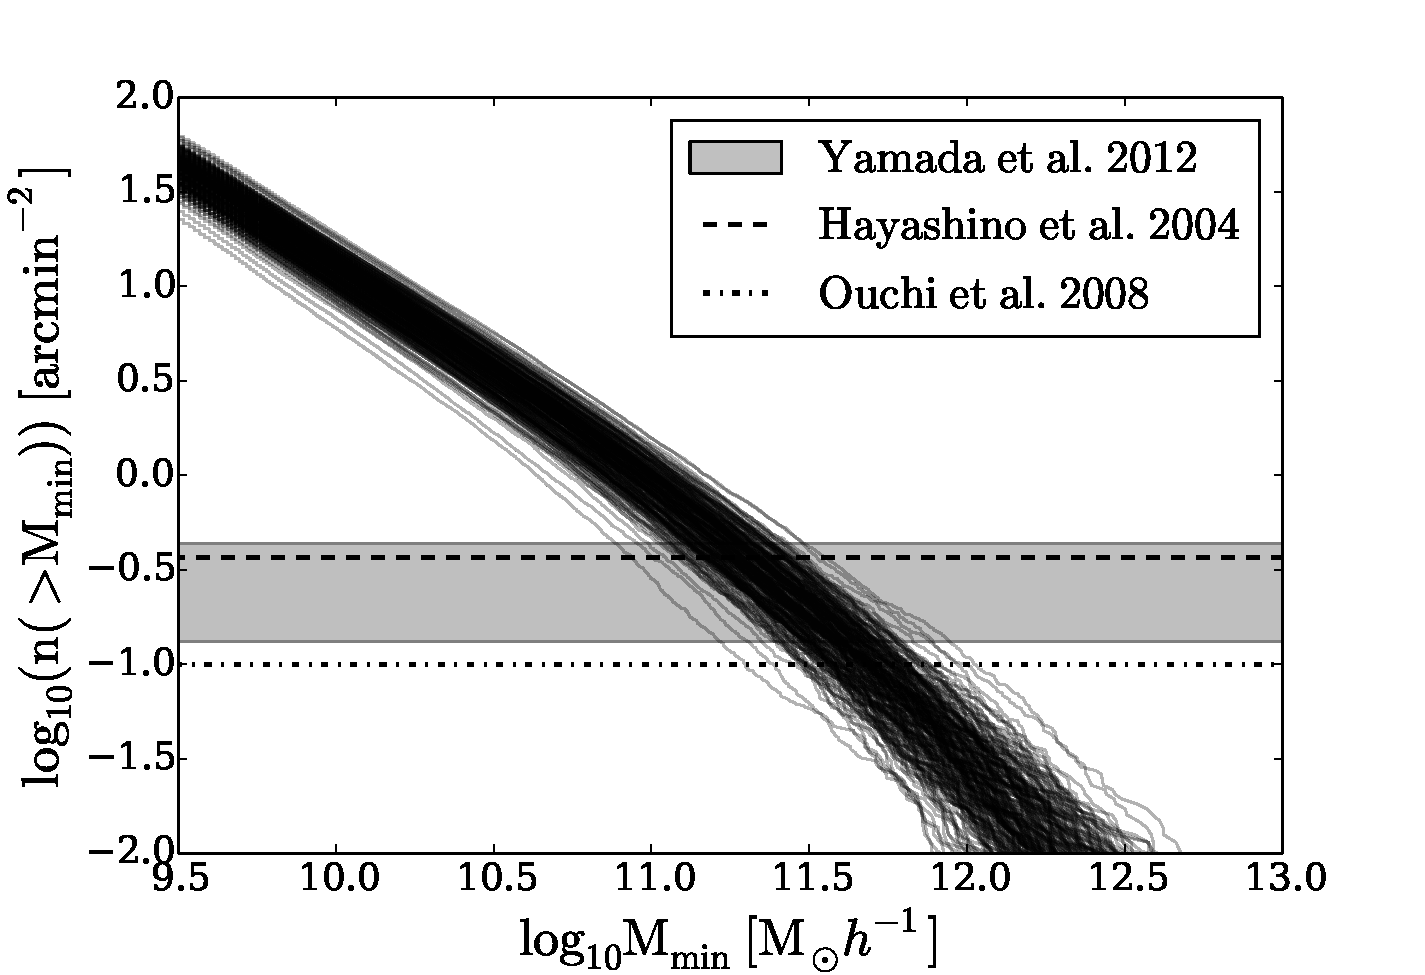
\includegraphics[width=0.95\linewidth,angle=0]{Fig1.pdf}
\caption{ \label{fig:halos} Surface density of dark 
  matter halos as a function of a minimum halo mass. Each line
  represents one of the $210$ volumes of dimensions $46\times 35\times
  41$ $h^{-3}$ Mpc$^{3}$ in the Bolshoi simulation. The horizontal
  gray band represents the range of surface densities observed for
  LAEs at $z=3.1$ as reported by \citet{Yamada2012} and the dashed
  line the observational results by \citet{Ouchi2008}.}
\end{center} 
\end{figure}


\begin{figure*}
\begin{center}
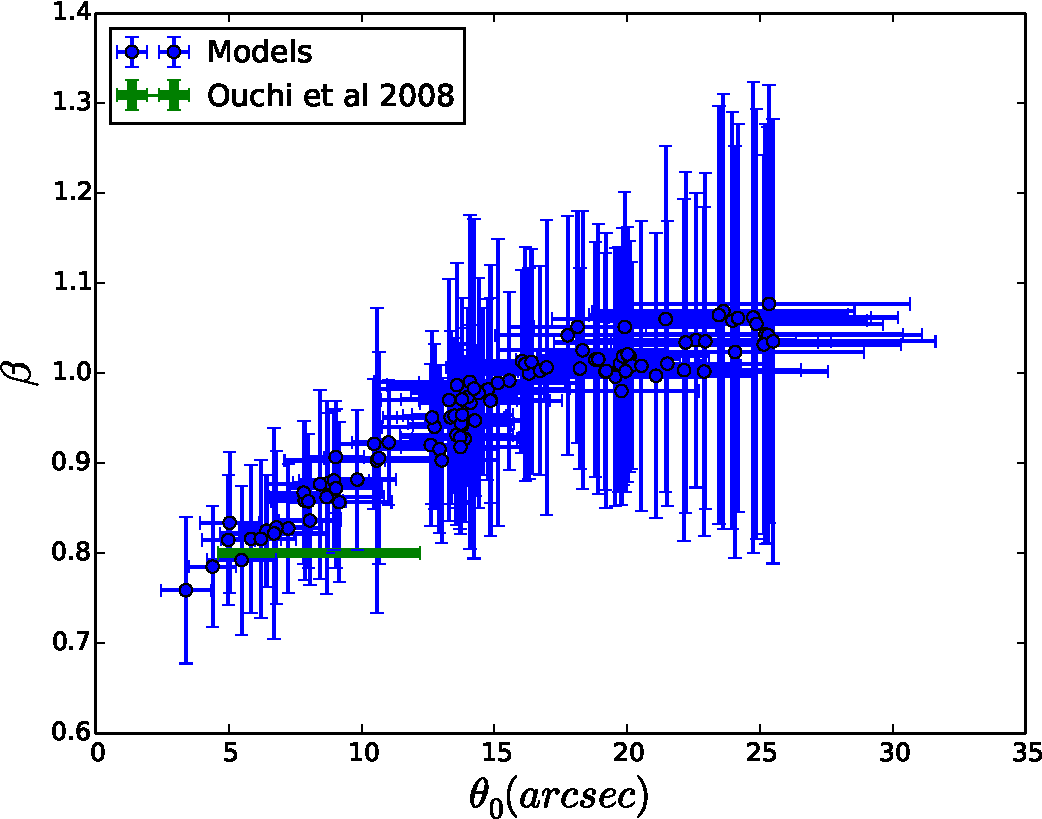
\includegraphics[width=0.49\linewidth,angle=0]{Fig7_corr_params.pdf}  
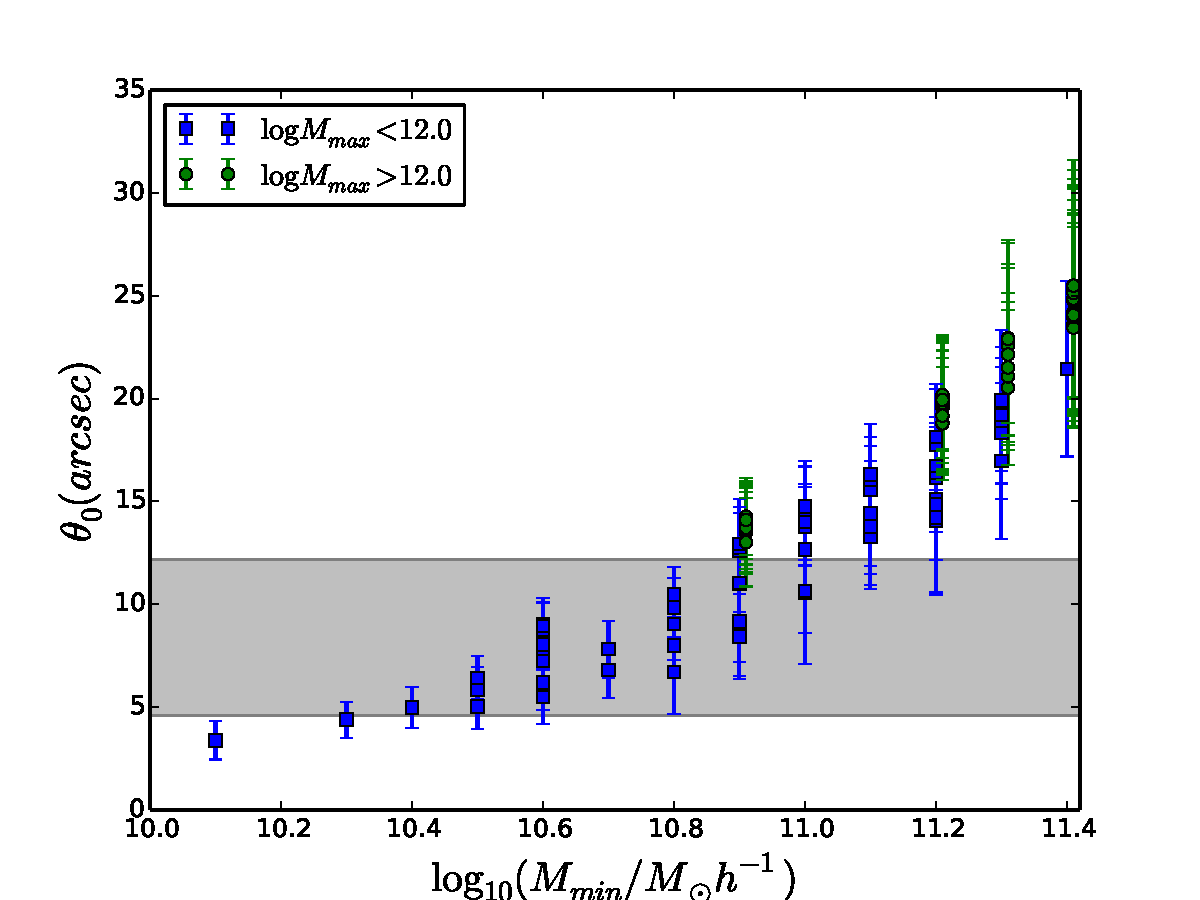
\includegraphics[width=0.49\linewidth,angle=0]{Fig7_mmin_vs_theta.pdf} 
\end{center}
\caption{Left panel. Values for the free parameters $\theta_{0}$ and $\beta$
in the fitting formula (Eq. \ref{eq:fitting}) for the angular
correlation function. Blue dots correspond to simulations and the
green line to observations by \citet{Ouchi2008,Ouchi2010}. The error
bars in the theoretical data correspond to the quadratic average of
the fitting uncertainties for each mock survey. Right panel. Values of
$\theta_{0}$  and $\log_{10}(M_{\rm min}/M_{\odot} h^{-1})$. Blue and
green point represents the models where  $\log_{10}(M_{\rm max}/M_{\odot}
h^{-1})<12.0$ and  $\log_{10}(M_{\rm min}/M_{\odot} h^{-1})>12.0$
respectively. .  The horizontal gray band represents the observational
constraints on $\theta_{0}$ established by
\citet{Ouchi2008,Ouchi2010}. Green points has been displaced by
$0.01$ dex of its original value to avoid overlapping between blue and
green points.} \label{fig:correlation_parameters}   
\end{figure*}


\subsection{Dark Matter Halo Number Density}

Figure \ref{fig:halos} shows the  integrated dark matter halo surface
density as a function of  minimum halo mass $M_{\rm min}$. Each line
corresponds to one of the 210 sub-volumes in the Bolshoi
simulation. The gray band indicates the surface density values for
LAEs allowed by observations \citep{Yamada2012}. The dashed lines
represent the values in the field observed by
\citep{Ouchi2008}. 

Figure \ref{fig:halos} illustrates the impact of cosmic variance. At a
fixed minimum mass there is an scatter of $0.3-0.6$ dex in the number
density abundance, which is of the same order of magnitude as the
scatter in the observational data. As a consequence the variation in
the number density in mocks for models with the same mass range and
occupation fraction can be by factors of $\sim 2-5$. 

 
Figure \ref{fig:halos} help us to understand why only a specific range of
models ${\mathcal M}$ can be expected to be consistent with
observations. From Figure \ref{fig:halos} we can read that models with
a minimum mass $M_{\rm min}>10^{12}$\hMsun always have a surface
number density lower than the observational constrain, making them
incompatible with observations; there are simply too few halos
compared to observed LAEs. The opposite is true in models with $M_{\rm
  min}<10^{11.0}$\hMsun, which have a surface number density larger
than observations. In those cases the maximum mass $M_{\rm max}$ and the
occupation fraction $f_{\rm occ}<1.0$  can be tuned in order to lower
the halo number density to match observations.    

\subsection{Maximally Consistent Models}


The left panel in Figure \ref{fig:correlation_parameters} shows the
results for the best estimates of $\theta_{0}$-$\beta$  used in the
ACF parametrization on the models that are already consistent with
the surface number density distribution.  Blue circles with error bars
represent the results from the mocks and the horizontal line the
observational results of \cite{Ouchi2008} over a field with average
number density where the $\beta$ parameter was fixed in the fit. From
this Figure we observe that there are models with too large values of
$\theta_0$ and/or $\beta$ that can be ruled out as inconsistent.

Figure \ref{fig:restriction_mock_and_f_occ_corr} presents the final
selection consistent models in the planes $M_{\rm min}$-$M_{\rm
  max}$ and $M_{\rm   min}$-$f_{\rm occ}$. We find that
we end up with $40$ models consistent with both the surface number
density constraints and the ACF.  This is a reduction of two orders of
magnitude with respect to the initial set of $9000$ models.

In the next section we review in detail these models and their
implications from the point of galaxy formation and other
constraints reported in the literature.

\section{Discussion}
\label{sec:discussion}

Out of the initial set of $9000$ models we end up with $40$ that are
consistent with the observational constraints. To facilitate the
discussion of these models we define a new quantity, the halo mass
range $\Delta M\equiv \log_{10}M_{\rm max} - \log_{10}M_{\rm  min}$, which
together with the occupation fraction, $f_{\rm occ}$, and the minimum
mass $M_{\rm min}$ allows us to classify all the successful models into
three families:     
  
\begin{itemize}
\item[(1)] Low occupation fraction $f_{\rm occ}\leq 0.2$ and narrow
  mass range $\Delta M\leq 1.0$ 
  dex: 16 models. 
\item[(2)] High occupation fraction $f_{\rm occ}> 0.2$ and
  narrow mass range $\Delta M\leq 1.0$: 17 models 
\item[(3)] Low occupation fraction $f_{\rm occ}\leq 0.2$ 
  and wide mass range $\Delta M>1.0$: 7 models
\end{itemize}

The models in the third family are barely consistent with the
constraints from the ACF. These models have another particular
feature: their minimum mass is exactly $M_{\rm min}=10^{10.9}\hMsun$
and $M_{\rm max}>10^{12.0}\hMsun$ . They have values of $\beta$
close to $1.0$ (instead of the observational value of $0.8$) and
$\theta_0$ on the range of $13^{\prime}$ (the mean observational
value is close to $8^{\prime}$) but are considered consistent
because their large error bars barely overlap with the observational
expectation (see figure \ref{fig:correlation_parameters}).
Because these models are barely compatible with observations and
are a minority of the consistent models, we exclude them from the
discussion.

\begin{figure*}
\begin{center}
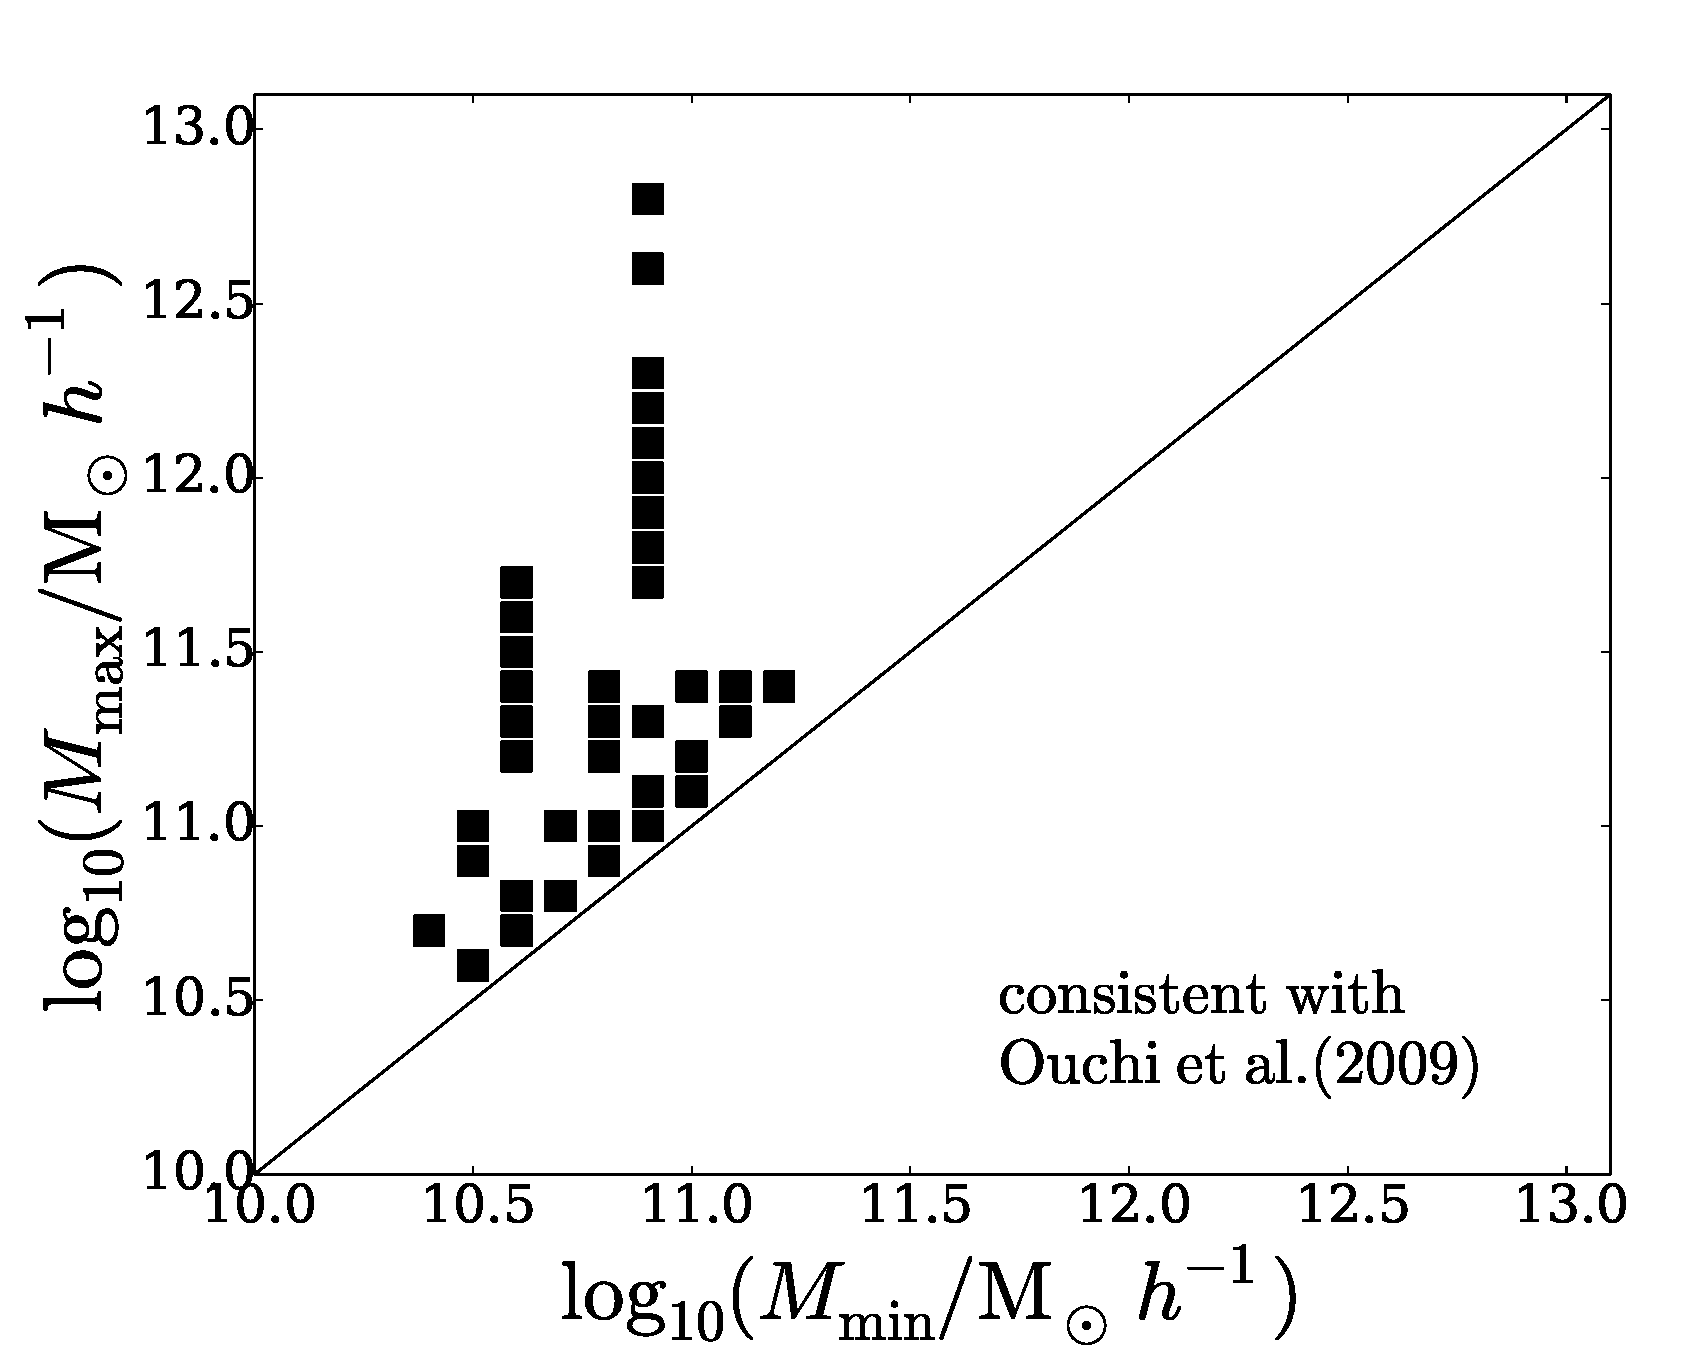
\includegraphics[width=0.49\linewidth,angle=0]{Fig6_mass.pdf}
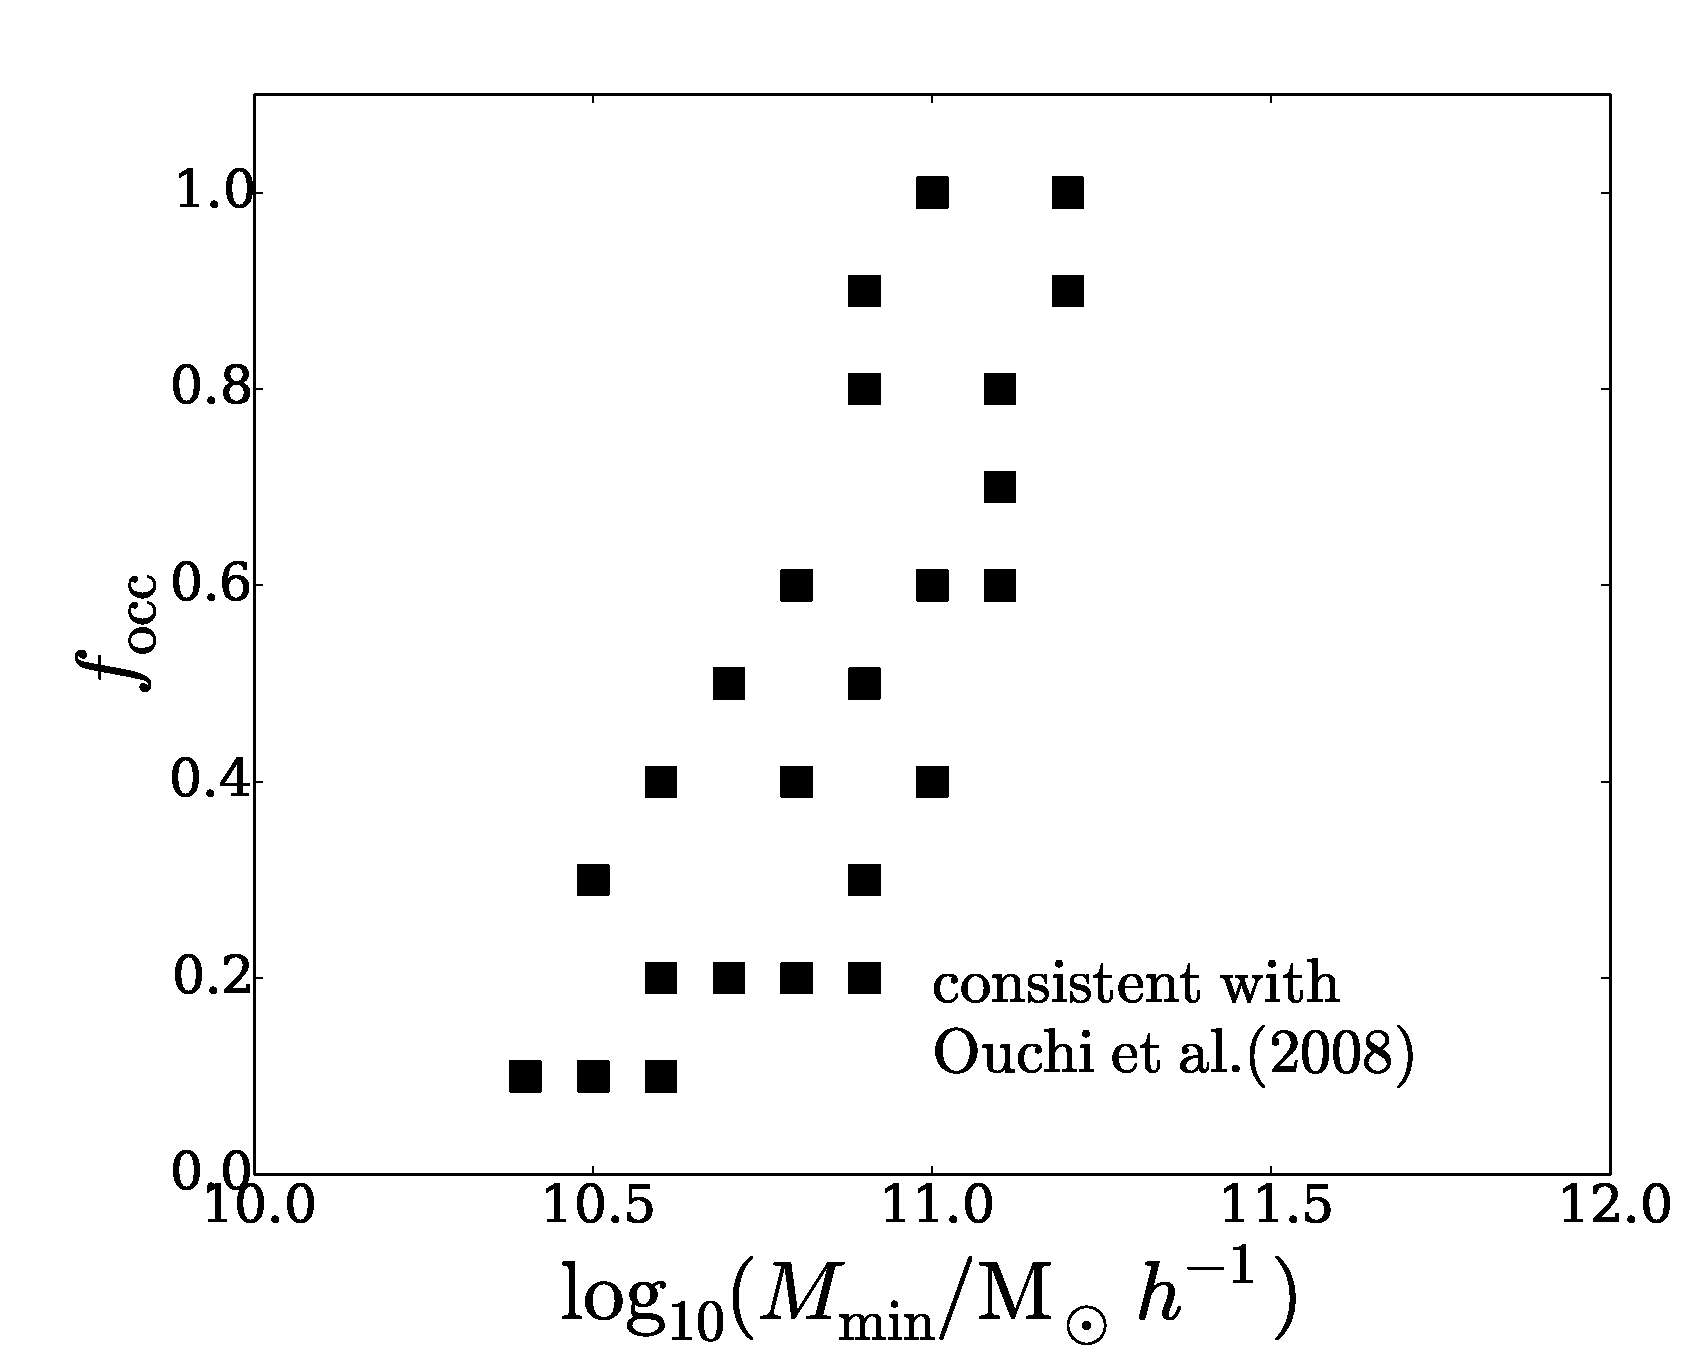
\includegraphics[width=0.49\linewidth,angle=0]{Fig6_f_occ.pdf}
\end{center} 
\caption{$M_{\rm min}$-$M_{\rm max}$ (left) and $M_{\rm
    min}$-$f_{\rm occ}$ (right) planes showing the models fulfilling both
   constraints on the maximal number of consistent mocks and the
  angular correlation function from \citet{Ouchi2008,Ouchi2010}.   
  \label{fig:restriction_mock_and_f_occ_corr}} 
\end{figure*} 


\subsection{Two relevant features in the preferred models}

There are two interesting features in the remaining two first
families. First, the occupation fraction can take any value from $0.1$
to $1.0$. Second, all constrained models of halos hosting LAEs 
 have a narrow mass range $\Delta M\leq 1.0$, and half of them 
 have $\Delta M\leq 0.5$.

The existence of models with high occupation fractions $f_{\rm
  occ}>0.2$ is unexpected from previous clustering analysis that do
not take  into account the effect of cosmic variance in the same way we
propose in this \documentname. Nevertheless, values of an occupation
fraction $f_{\rm occ}=0.1$ and the mass range predicted by all of our
models are consistent with already published observational results
\citep{Gawiser07,Ouchi2010}. This suggests that explicitly taking
cosmic variance of the observed fields into account (the only point
not included in the analysis already cited) hinders the possibility of
constraining the LAEs occupation fraction. 

Concerning the narrow mass range $\Delta M <1.0$ the question arises
of how can we give a physical interpretation for the existence of such
a narrow mass range. We can start with a reasonable
assumption. Namely, that the star formation rate increases with halo's
mass. Under this assumption the cut at the low mass end, $M_{\rm
  min}$, can be interpreted in terms of the minimal star formation
rate required to produce a \ly luminosity above observational
detection thresholds.   A cut at higher halo masses $M_{\rm  max}$
requires a different justification. There are two complementary
physical scenarios that could provide it. 

One scenario can be presented in terms of a decreasing escape fraction
of \ly radiation in massive systems. Detailed galaxy formation models
support the idea that massive galaxies with higher metallicities have
larger dust contents and a less concentrated ISM than lower mass
systems. Due to the resonant nature of the \ly line the probability of
absorption  of \ly photons increases in massive systems, producing
high absorption of the \ly line but not of UV continuum or other
non-resonant lines \citep{Laursen2009,ForeroRomero2011}. In a second
scenario larger systems have more extended gaseous envelopes which due
to resonance effects of the \ly line, induces a low surface brightness
and a broader line, making these systems less observable in narrow
band filter surveys \citep{Laursen2009,Zheng2010}.    

\subsection{Comparison to previous clustering estimates}

Observational evidence based on the ACF inferred from photometric
measurements in the Extended Chandra Deep Field South has shown that
the median dark matter masses of halos hosting LAEs is
$\log_{10}M_{\rm  med}=10.9^{+0.5}_{-0.9}$\Msun, with a corresponding
occupation fraction of $1-10\%$  \citep{Gawiser07}.  \cite{Ouchi2010}
presents analysis of LAE observations in the redshift interval
$3.1<z<7.0$ and at $z=3.1$ They quote an average mass for the host
dark matter halos of $M_{h}=2.9^{+24.0}_{-2.9}\times 10^{10}$ \hMsun
with a corresponding duty cycle of $0.008\pm 0.03$.  

Our results are in a general good agreement with those estimates for
the host mass and the upper limit of the occupation fraction. This is
not completely unexpected given that we have also required consistency
with ACF measurements. These expectations are mostly matched by
the first family of models which favor only the  low
($\sim 10\%$) occupations fractions, are also consistent in that
regard with the observational expectations by \cite{Gawiser07}. 

The novelty in our results is that we have a detailed estimate for 
host halo mass range together with the occupation fraction. This allows us
to show that the halo mass range can, in some cases, be narrow $\Delta M <
0.3$ dex, something that cannot be inferred from ACF analysis alone.
Furthermore, In contrast to \cite{Gawiser07} and \cite{Ouchi2010} we
find that an ACF analysis is not enough to rule out models with a high
occupation fraction $f_{\rm occ}>0.1$. 

\section{Conclusions}
\label{sec:conclusions}

In this \documentname constrained the  mass and occupation fraction of dark matter halos
hosting Lyman $\alpha$ Emitters at redshift $z=3.1$ taking into
account cosmic variance in a $\Lambda$CDM cosmology.  To this end we built a large number of mock catalogs
matching observational geometries. The mocks were constructed from a
N-body simulation by assigning a single LAE to a DM halo.
 
We proceeded with a thorough exploration of the parameter space
($M_{\rm min}$, $M_{\rm max}$, $f_{\rm occ}$) describing our
model. We looked for consistency with two observational constraints: the
surface number density distribution and the angular correlation
function. Out of the initial $9000$  combinations of parameters in the
model we found $40$ consistent with observations.  The minimum mass and
maximum mass of these consistent models were found to be in the
ranges:   $M_{\rm  max}<10^{12}$\hMsun\ and $10^{10.2}\hMsun\leq
M_{\rm min}\leq 10^{11.5}\hMsun$.  This supports the notion that the
most massive halos at $z=3.1$ do not host detectable LAEs.  

We found two interesting features in these models. First, the
occupation fraction remains unconstrained; second, many models have a
narrow mass range models with $\Delta M \leq 0.5$.   
 
The wide range of occupation fraction values is unexpected from
previous studies \citep[i.e.][]{Gawiser2007,Ouchi2010}  that
unanimously favor low values on the range of $10^{-2}$ and only
consider values of $0.1$ as an upper limit. Nevertheless, all the halo
mass ranges deduced in previous analysis are a subset of the models we
found with our method. 

We consider that putting tight constraints on the occupation cannot be
done from spatial information only. This requires additional modeling and
larger observed fields to narrow down the link between halo mass, star
formation and escaping \ly radiation. Additionally, the narrow halo
mass range for halos hosting LAEs can be seen as an additional
constraint for galaxy formation models that hope to address these
questions. 

From the point of view of Dark Energy surveys such as the Hobby-Eberly
Telescope Dark Enery Experiment (HETDEX) the narrow mass range for
LAEs can be seen as an advantage because its simplicity in their
modeling aiming at recovering cosmological parameters. We foresee that
the observations with new instruments (such as the Multi Unit
Spectroscopic Explorer (MUSE), Hyper SuprimeCam and HETDEX) covering
more fields and a wider range of luminosities will be key in fully
understanding the effects of cosmic variance  and imposing tighter
constraints on the properties of dark matter halos hosting LAEs. 



\section*{Acknowledgments} 

J.E.F-R was supported by the FAPA grant by Vicerrector\'ia de
Investigaciones at Universidad de los Andes.  

J.E.F-R thanks the hospitality of Changbom Park and the Korea
Institute for Advanced Study where the first full draft of this paper
was completed. The authors also thank Peter Laursen, Paulina Lira, 
Alvaro Orsi and Mark Dijkstra for helpful comments on the physical
interpretation and presentation of our results. 


The MultiDark Database used in this paper and the web application
providing online access to it were constructed as part of the
activities of the German Astrophysical Virtual Observatory as result
of a collaboration between the Leibniz-Institute for Astrophysics
Potsdam (AIP) and the Spanish MultiDark Consolider Project
CSD2009-00064. The Bolshoi and MultiDark simulations were run on the
NASA's Pleiades supercomputer at the NASA Ames Research Center. 



\bibliographystyle{apj}
%\bibliography{references}
\begin{thebibliography}{36}
\expandafter\ifx\csname natexlab\endcsname\relax\def\natexlab#1{#1}\fi

\bibitem[{{Behroozi} {et~al.}(2013){Behroozi}, {Wechsler}, \&
  {Conroy}}]{Behroozi2013a}
{Behroozi}, P.~S., {Wechsler}, R.~H., \& {Conroy}, C. 2013, \apj, 770, 57

\bibitem[{{Bond} {et~al.}(2009){Bond}, {Gawiser}, {Gronwall}, {Ciardullo},
  {Altmann}, \& {Schawinski}}]{Bond2009}
{Bond}, N.~A., {Gawiser}, E., {Gronwall}, C., {Ciardullo}, R., {Altmann}, M.,
  \& {Schawinski}, K. 2009, \apj, 705, 639

\bibitem[{{Colberg} {et~al.}(2000){Colberg}, {White}, {Yoshida}, {MacFarland},
  {Jenkins}, {Frenk}, {Pearce}, {Evrard}, {Couchman}, {Efstathiou}, {Peacock},
  {Thomas}, \& {Virgo Consortium}}]{Colberg00}
{Colberg}, J.~M., {White}, S.~D.~M., {Yoshida}, N., {MacFarland}, T.~J.,
  {Jenkins}, A., {Frenk}, C.~S., {Pearce}, F.~R., {Evrard}, A.~E., {Couchman},
  H.~M.~P., {Efstathiou}, G., {Peacock}, J.~A., {Thomas}, P.~A., \& {Virgo
  Consortium}. 2000, \mnras, 319, 209

\bibitem[{{Dayal} {et~al.}(2009){Dayal}, {Ferrara}, {Saro}, {Salvaterra},
  {Borgani}, \& {Tornatore}}]{Dayal2009}
{Dayal}, P., {Ferrara}, A., {Saro}, A., {Salvaterra}, R., {Borgani}, S., \&
  {Tornatore}, L. 2009, \mnras, 400, 2000

\bibitem[{{Dijkstra} \& {Kramer}(2012)}]{Dijkstra2012}
{Dijkstra}, M., \& {Kramer}, R. 2012, \mnras, 424, 1672

\bibitem[{{Dijkstra} {et~al.}(2011){Dijkstra}, {Mesinger}, \&
  {Wyithe}}]{Dijkstra11}
{Dijkstra}, M., {Mesinger}, A., \& {Wyithe}, J.~S.~B. 2011, \mnras, 414, 2139

\bibitem[{{Forero-Romero} {et~al.}(2011){Forero-Romero}, {Yepes},
  {Gottl{\"o}ber}, {Knollmann}, {Cuesta}, \& {Prada}}]{ForeroRomero2011}
{Forero-Romero}, J.~E., {Yepes}, G., {Gottl{\"o}ber}, S., {Knollmann}, S.~R.,
  {Cuesta}, A.~J., \& {Prada}, F. 2011, \mnras, 415, 3666

\bibitem[{{Forero-Romero} {et~al.}(2012){Forero-Romero}, {Yepes},
  {Gottl{\"o}ber}, \& {Prada}}]{ForeroRomero2012}
{Forero-Romero}, J.~E., {Yepes}, G., {Gottl{\"o}ber}, S., \& {Prada}, F. 2012,
  \mnras, 419, 952

\bibitem[{{Garel} {et~al.}(2012){Garel}, {Blaizot}, {Guiderdoni}, {Schaerer},
  {Verhamme}, \& {Hayes}}]{Garel2012}
{Garel}, T., {Blaizot}, J., {Guiderdoni}, B., {Schaerer}, D., {Verhamme}, A.,
  \& {Hayes}, M. 2012, \mnras, 422, 310

\bibitem[{{Gawiser} {et~al.}(2007{\natexlab{a}}){Gawiser}, {Francke}, {Lai},
  {Schawinski}, {Gronwall}, {Ciardullo}, {Quadri}, {Orsi}, {Barrientos},
  {Blanc}, {Fazio}, \& {Feldmeier}}]{Gawiser2007}
{Gawiser}, E., {Francke}, H., {Lai}, K., {Schawinski}, K., {Gronwall}, C.,
  {Ciardullo}, R., {Quadri}, R., {Orsi}, A., {Barrientos}, L.~F., {Blanc},
  G.~A., {Fazio}, G., \& {Feldmeier}, J.~J. 2007{\natexlab{a}}, \apj, 671, 278

\bibitem[{{Gawiser} {et~al.}(2007{\natexlab{b}}){Gawiser}, {Francke}, {Lai},
  {Schawinski}, {Gronwall}, {Ciardullo}, {Quadri}, {Orsi}, {Barrientos},
  {Blanc}, {Fazio}, {Feldmeier}, {Huang}, {Infante}, {Lira}, \&
  {Padilla}}]{Gawiser07}
{Gawiser}, E., {Francke}, H., {Lai}, K., {Schawinski}, K., {Gronwall}, C.,
  {Ciardullo}, R., {Quadri}, R., {Orsi}, A., {Barrientos}, L.~F., {Blanc},
  G.~A., {Fazio}, G., {Feldmeier}, J.~J., {Huang}, J.-s., {Infante}, L.,
  {Lira}, P., \& {Padilla}, N. 2007{\natexlab{b}}, \apj, 671, 278

\bibitem[{{Gronwall} {et~al.}(2007){Gronwall}, {Ciardullo}, {Hickey},
  {Gawiser}, {Feldmeier}, {van Dokkum}, {Urry}, {Herrera}, {Lehmer}, {Infante},
  {Orsi}, {Marchesini}, {Blanc}, {Francke}, {Lira}, \& {Treister}}]{Gronwall07}
{Gronwall}, C., {Ciardullo}, R., {Hickey}, T., {Gawiser}, E., {Feldmeier},
  J.~J., {van Dokkum}, P.~G., {Urry}, C.~M., {Herrera}, D., {Lehmer}, B.~D.,
  {Infante}, L., {Orsi}, A., {Marchesini}, D., {Blanc}, G.~A., {Francke}, H.,
  {Lira}, P., \& {Treister}, E. 2007, \apj, 667, 79

\bibitem[{{Guaita} {et~al.}(2013){Guaita}, {Francke}, {Gawiser}, {Bauer},
  {Hayes}, {{\"O}stlin}, \& {Padilla}}]{Guaita2013}
{Guaita}, L., {Francke}, H., {Gawiser}, E., {Bauer}, F.~E., {Hayes}, M.,
  {{\"O}stlin}, G., \& {Padilla}, N. 2013, \aap, 551, A93

\bibitem[{{Hayashino} {et~al.}(2004){Hayashino}, {Matsuda}, {Tamura},
  {Yamauchi}, {Yamada}, {Ajiki}, {Fujita}, {Murayama}, {Nagao}, {Ohta},
  {Okamura}, {Ouchi}, {Shimasaku}, {Shioya}, \& {Taniguchi}}]{Hayashino2004}
{Hayashino}, T., {Matsuda}, Y., {Tamura}, H., {Yamauchi}, R., {Yamada}, T.,
  {Ajiki}, M., {Fujita}, S.~S., {Murayama}, T., {Nagao}, T., {Ohta}, K.,
  {Okamura}, S., {Ouchi}, M., {Shimasaku}, K., {Shioya}, Y., \& {Taniguchi}, Y.
  2004, \aj, 128, 2073

\bibitem[{{Hinshaw} {et~al.}(2013){Hinshaw}, {Larson}, {Komatsu}, {Spergel},
  {Bennett}, {Dunkley}, {Nolta}, {Halpern}, {Hill}, {Odegard}, {Page}, {Smith},
  {Weiland}, {Gold}, {Jarosik}, {Kogut}, {Limon}, {Meyer}, {Tucker}, {Wollack},
  \& {Wright}}]{hinshaw_etal13}
{Hinshaw}, G., {Larson}, D., {Komatsu}, E., {Spergel}, D.~N., {Bennett}, C.~L.,
  {Dunkley}, J., {Nolta}, M.~R., {Halpern}, M., {Hill}, R.~S., {Odegard}, N.,
  {Page}, L., {Smith}, K.~M., {Weiland}, J.~L., {Gold}, B., {Jarosik}, N.,
  {Kogut}, A., {Limon}, M., {Meyer}, S.~S., {Tucker}, G.~S., {Wollack}, E., \&
  {Wright}, E.~L. 2013, \apjs, 208, 19

\bibitem[{{Jose} {et~al.}(2013){Jose}, {Srianand}, \&
  {Subramanian}}]{Jose2013b}
{Jose}, C., {Srianand}, R., \& {Subramanian}, K. 2013, ArXiv e-prints

\bibitem[{{Klypin} {et~al.}(2011){Klypin}, {Trujillo-Gomez}, \&
  {Primack}}]{Bolshoi}
{Klypin}, A.~A., {Trujillo-Gomez}, S., \& {Primack}, J. 2011, \apj, 740, 102

\bibitem[{{Koehler} {et~al.}(2007){Koehler}, {Schuecker}, \&
  {Gebhardt}}]{Koehler2007}
{Koehler}, R.~S., {Schuecker}, P., \& {Gebhardt}, K. 2007, \aap, 462, 7

\bibitem[{{Kudritzki} {et~al.}(2000){Kudritzki}, {M{\'e}ndez}, {Feldmeier},
  {Ciardullo}, {Jacoby}, {Freeman}, {Arnaboldi}, {Capaccioli}, {Gerhard}, \&
  {Ford}}]{Kudritzki2000}
{Kudritzki}, R.-P., {M{\'e}ndez}, R.~H., {Feldmeier}, J.~J., {Ciardullo}, R.,
  {Jacoby}, G.~H., {Freeman}, K.~C., {Arnaboldi}, M., {Capaccioli}, M.,
  {Gerhard}, O., \& {Ford}, H.~C. 2000, \apj, 536, 19

\bibitem[{{Landy} \& {Szalay}(1993)}]{Landy1993}
{Landy}, S.~D., \& {Szalay}, A.~S. 1993, \apj, 412, 64

\bibitem[{{Laursen} {et~al.}(2013){Laursen}, {Duval}, \&
  {{\"O}stlin}}]{Laursen2013}
{Laursen}, P., {Duval}, F., \& {{\"O}stlin}, G. 2013, \apj, 766, 124

\bibitem[{{Laursen} {et~al.}(2009){Laursen}, {Razoumov}, \&
  {Sommer-Larsen}}]{Laursen2009}
{Laursen}, P., {Razoumov}, A.~O., \& {Sommer-Larsen}, J. 2009, \apj, 696, 853

\bibitem[{{Laursen} \& {Sommer-Larsen}(2007)}]{Laursen2007}
{Laursen}, P., \& {Sommer-Larsen}, J. 2007, \apjl, 657, L69

\bibitem[{{Matsuda} {et~al.}(2005){Matsuda}, {Yamada}, {Hayashino}, {Tamura},
  {Yamauchi}, {Murayama}, {Nagao}, {Ohta}, {Okamura}, {Ouchi}, {Shimasaku},
  {Shioya}, \& {Taniguchi}}]{Matsuda2005}
{Matsuda}, Y., {Yamada}, T., {Hayashino}, T., {Tamura}, H., {Yamauchi}, R.,
  {Murayama}, T., {Nagao}, T., {Ohta}, K., {Okamura}, S., {Ouchi}, M.,
  {Shimasaku}, K., {Shioya}, Y., \& {Taniguchi}, Y. 2005, \apjl, 634, L125

\bibitem[{{Neufeld}(1991)}]{Neufeld1991}
{Neufeld}, D.~A. 1991, \apjl, 370, L85

\bibitem[{{Nilsson} {et~al.}(2007){Nilsson}, {M{\o}ller}, {M{\"o}ller},
  {Fynbo}, {Micha{\l}owski}, {Watson}, {Ledoux}, {Rosati}, {Pedersen}, \&
  {Grove}}]{Nilsson2007}
{Nilsson}, K.~K., {M{\o}ller}, P., {M{\"o}ller}, O., {Fynbo}, J.~P.~U.,
  {Micha{\l}owski}, M.~J., {Watson}, D., {Ledoux}, C., {Rosati}, P.,
  {Pedersen}, K., \& {Grove}, L.~F. 2007, \aap, 471, 71

\bibitem[{{Orsi} {et~al.}(2012){Orsi}, {Lacey}, \& {Baugh}}]{Orsi2012}
{Orsi}, A., {Lacey}, C.~G., \& {Baugh}, C.~M. 2012, \mnras, 425, 87

\bibitem[{{Ouchi} {et~al.}(2008){Ouchi}, {Shimasaku}, {Akiyama}, {Simpson},
  {Saito}, {Ueda}, {Furusawa}, {Sekiguchi}, {Yamada}, {Kodama}, {Kashikawa},
  {Okamura}, {Iye}, {Takata}, {Yoshida}, \& {Yoshida}}]{Ouchi2008}
{Ouchi}, M., {Shimasaku}, K., {Akiyama}, M., {Simpson}, C., {Saito}, T.,
  {Ueda}, Y., {Furusawa}, H., {Sekiguchi}, K., {Yamada}, T., {Kodama}, T.,
  {Kashikawa}, N., {Okamura}, S., {Iye}, M., {Takata}, T., {Yoshida}, M., \&
  {Yoshida}, M. 2008, \apjs, 176, 301

\bibitem[{{Ouchi} {et~al.}(2010){Ouchi}, {Shimasaku}, {Furusawa}, {Saito},
  {Yoshida}, {Akiyama}, {Ono}, {Yamada}, {Ota}, {Kashikawa}, {Iye}, {Kodama},
  {Okamura}, {Simpson}, \& {Yoshida}}]{Ouchi2010}
{Ouchi}, M., {Shimasaku}, K., {Furusawa}, H., {Saito}, T., {Yoshida}, M.,
  {Akiyama}, M., {Ono}, Y., {Yamada}, T., {Ota}, K., {Kashikawa}, N., {Iye},
  M., {Kodama}, T., {Okamura}, S., {Simpson}, C., \& {Yoshida}, M. 2010, \apj,
  723, 869

\bibitem[{{Peebles}(1980)}]{Peebles1980}
{Peebles}, P.~J.~E. 1980, {The large-scale structure of the universe}

\bibitem[{Riebe {et~al.}(2013)Riebe, Partl, Enke, Forero-Romero, Gottlöber,
  Klypin, Lemson, Prada, Primack, Steinmetz, \& Turchaninov}]{MultiDark}
Riebe, K., Partl, A.~M., Enke, H., Forero-Romero, J., Gottlöber, S., Klypin,
  A., Lemson, G., Prada, F., Primack, J.~R., Steinmetz, M., \& Turchaninov, V.
  2013, Astronomische Nachrichten, 334, 691

\bibitem[{{Springel} {et~al.}(2005){Springel}, {White}, {Jenkins}, {Frenk},
  {Yoshida}, {Gao}, {Navarro}, {Thacker}, {Croton}, {Helly}, {Peacock}, {Cole},
  {Thomas}, {Couchman}, {Evrard}, {Colberg}, \& {Pearce}}]{SpringelNature05}
{Springel}, V., {White}, S.~D.~M., {Jenkins}, A., {Frenk}, C.~S., {Yoshida},
  N., {Gao}, L., {Navarro}, J., {Thacker}, R., {Croton}, D., {Helly}, J.,
  {Peacock}, J.~A., {Cole}, S., {Thomas}, P., {Couchman}, H., {Evrard}, A.,
  {Colberg}, J., \& {Pearce}, F. 2005, \nat, 435, 629

\bibitem[{{Verhamme} {et~al.}(2006){Verhamme}, {Schaerer}, \&
  {Maselli}}]{Verhamme2006}
{Verhamme}, A., {Schaerer}, D., \& {Maselli}, A. 2006, \aap, 460, 397

\bibitem[{{Yajima} {et~al.}(2012){Yajima}, {Choi}, \& {Nagamine}}]{Yajima2012}
{Yajima}, H., {Choi}, J.-H., \& {Nagamine}, K. 2012, \mnras, 427, 2889

\bibitem[{{Yamada} {et~al.}(2012){Yamada}, {Nakamura}, {Matsuda}, {Hayashino},
  {Yamauchi}, {Morimoto}, {Kousai}, \& {Umemura}}]{Yamada2012}
{Yamada}, T., {Nakamura}, Y., {Matsuda}, Y., {Hayashino}, T., {Yamauchi}, R.,
  {Morimoto}, N., {Kousai}, K., \& {Umemura}, M. 2012, \aj, 143, 79

\bibitem[{{Zheng} {et~al.}(2010){Zheng}, {Cen}, {Trac}, \&
  {Miralda-Escud{\'e}}}]{Zheng2010}
{Zheng}, Z., {Cen}, R., {Trac}, H., \& {Miralda-Escud{\'e}}, J. 2010, \apj,
  716, 574

\end{thebibliography}

\end{document}
